\begin{tikzpicture}

	\onslide<1->{\node[inner sep=0pt] (A) at (-5,9) {
\includegraphics[scale=0.45]{images/12.JPG}};}
	\onslide<2->{\node[inner sep=0pt] (A) at (-2.5,9) {
\includegraphics[scale=0.1]{images/plus.png}};}
	
	\onslide<3->{\node[inner sep=0pt] (A) at (0,9) {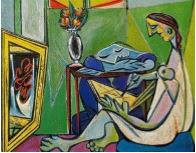
\includegraphics[scale=0.6]{images/11.JPG}};}
	
	\onslide<4->{\node[inner sep=0pt] (A) at (2.5,9) {
\includegraphics[scale=0.1]{images/equal.png}};}
	
	\onslide<5->{\node[inner sep=0pt] (A) at (5,9) {
\includegraphics[scale=0.45]{images/13.JPG}};}

\end{tikzpicture}